% -*- coding: utf-8 -*-

\section{Gradient Boost Decision Tree (GBDT)}
% http://nbviewer.jupyter.org/github/facaiy/book_notes/blob/master/machine_learning/tree/gbdt/intro.ipynb
% http://nbviewer.jupyter.org/github/facaiy/book_notes/blob/master/machine_learning/tree/gbdt/spark/intro.ipynb
\subsection{直观印象}
% 模型叠加
% 残差
\begin{frame}
    \begin{figure}[!tb]
        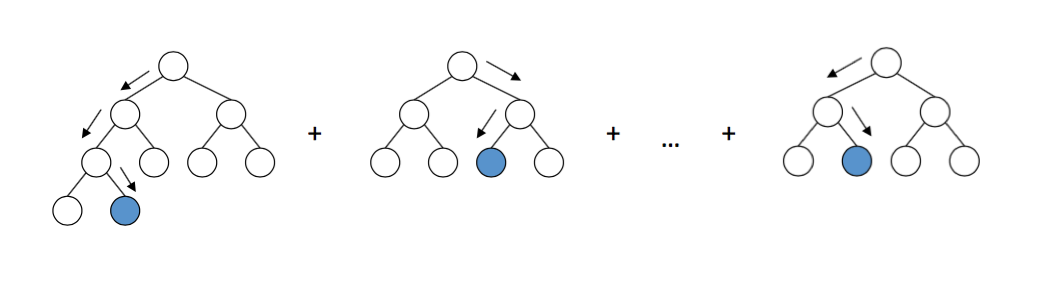
\includegraphics[width=1.2\onepicwidth]{figure/gbdt/gbdt_attractive_picture}
        \caption{GBDT示意\footnote{
                 \href{http://arogozhnikov.github.io/2016/06/24/gradient_boosting_explained.html}{Gradient Boosting explained, Alex Rogozhnikov}}}
    \end{figure}
\end{frame}


\subsection{算法流程}
\begin{frame}
    \begin{figure}[!tb]
        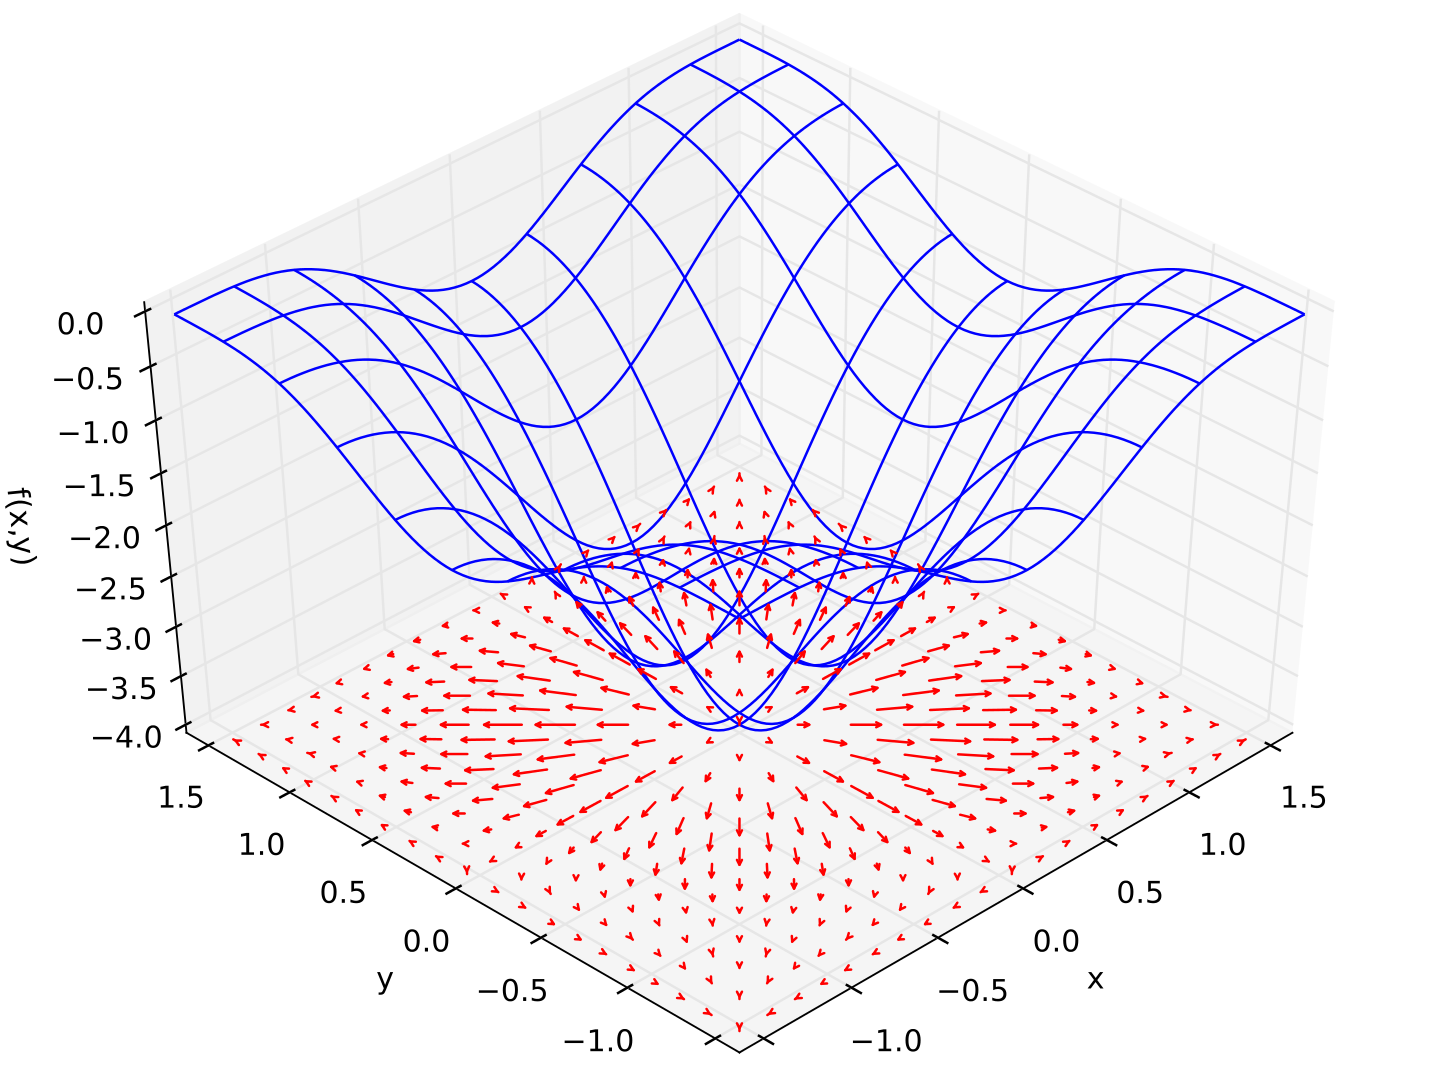
\includegraphics[width=\onepicwidth]{figure/gbdt/Gradient_Visual}
        \caption{损失函数示意\footnote{
                 \href{https://en.wikipedia.org/wiki/File:Gradient_Visual.svg}{Gradient Visual, Wikipedia}}}
    \end{figure}
\end{frame}

% https://en.wikipedia.org/wiki/Gradient_boosting
%% greedy: pdf, Algorithm 1
\begin{frame}
    \begin{algorithm}[H]
        $F_0(x) = \operatorname{arg \, min}_\rho \sum_{i=1}^N L(y_i, \rho)$ \;
        \For{$m=1$ \KwTo $M$}{
            $\tilde{y} = - \left [ \frac{\partial L (y_i, F(x_i))}{\partial F(x_i)} \right ]_{F(x) = F_{m-1}(x)}, \quad i = 1, 2, \dotsc, N$ \;
            $\mathbf{a}_m = \operatorname{arg \, min}_{\mathbf{a}, \beta} \sum_{i=1}^N \left [ \tilde{y}_i - \beta h(x_i; \mathbf{a}) \right ]^2$ \;
            $\rho_m = \operatorname{arg \, min}_\rho \sum_{i=1}^N L \left ( y_i, F_{m-1}(x_i) + \rho h(x_i; \mathbf{a}_m) \right)$ \;
            $F_m(x) = F_{m-1}(x) + \rho_m h(x; \mathbf{a}_m)$ \;
        }
        \caption{Gradient\_Boost}
    \end{algorithm}
    {\tiny Greedy function approximation: A gradient boosting machine, Jerome H. Friedman}
\end{frame}


\subsection{从最优化角度的理解}
% 从最速下降法来理解
%% L(,) 距离函数
%% 一维 U
%% 二维 曲面
\begin{frame}
    \begin{figure}
        \centering
        \subfigure[][]{
            \resizebox{0.53\linewidth}{!}{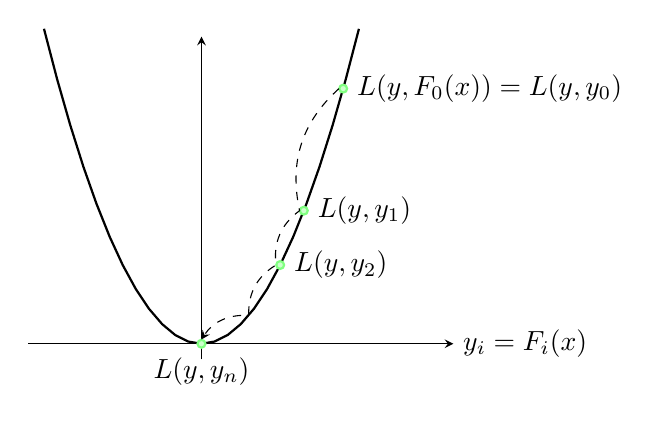
\begin{tikzpicture}
    [place/.style={circle,scale=0.3,draw=green!50,fill=green!20,thick},
    transition/.style={rectangle,draw=black!50,fill=black!20,thick}]

    %\draw[help lines] (-2.9,-0.2) grid (2.9,3.9);
    \draw[->,>=stealth] (-2.2,0) -- (3.2,0) node[right] {$y_i=F_i(x)$};
    \draw[->,>=stealth] (0,-0.2) -- (0,3.9);
    \draw[thick,color=black,domain=-2:2] plot (\x,\x*\x);

    \node[place,label=right:{$L(y,F_0(x)) = L(y, y_0)$}] (f0) at (1.8,3.24)  {};
    \node[place,label=right:{$L(y,y_1)$}] (f1) at (1.3,1.69)  {};
    \node[place,label=right:{$L(y,y_2)$}] (f2) at (1.0,1.0)   {};
    \node[place,label=below:{$L(y,y_n)$}] (fn) at (0,0)  {};

    \draw[->,>=stealth,dashed] (f0.west) to[bend right] (f1.west)
          to[bend right] (f2.west)
          to[bend right] (0.6,0.36)
          to[bend right] (fn.north);
\end{tikzpicture}
}
        }
        \hfil
        \subfigure[][]{
            \resizebox{0.40\linewidth}{!}{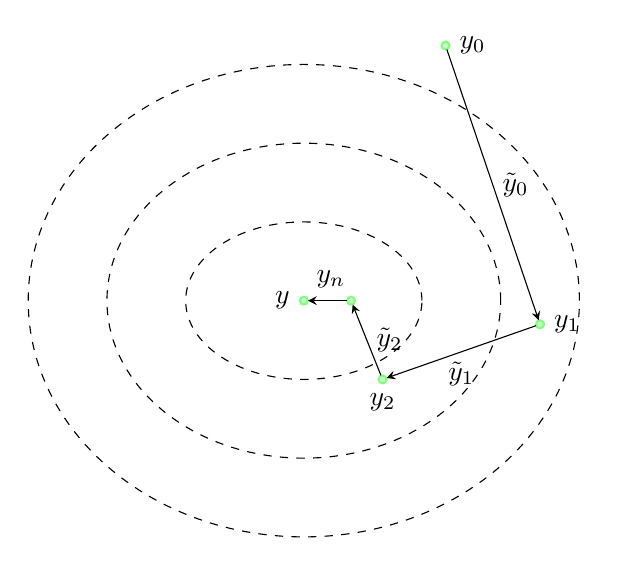
\begin{tikzpicture}
    [place/.style={circle,scale=0.3,draw=green!50,fill=green!20,thick},
    transition/.style={rectangle,draw=black!50,fill=black!20,thick}]

    %\draw[help lines] (-2.9,-0.2) grid (2.9,3.9);
    \draw[dashed] (0,0) circle [x radius=1.5, y radius=1];
    \draw[dashed] (0,0) circle [x radius=2.5, y radius=2];
    \draw[dashed] (0,0) circle [x radius=3.5, y radius=3];
    %\draw[dashed,thin] (0,0) circle [x radius=4.5, y radius=4];

    \node[place,label=right:{$y_0$}] (f0) at (1.8,3.24)  {};
    \node[place,label=right:{$y_1$}] (f1) at (3.0,-0.3)  {};
    \node[place,label=below:{$y_2$}] (f2) at (1.0,-1.0)   {};
    \node[place] (f3) at (0.6,0.0)   {};
    \node[place,label=left:{$y$},label=north east:{$y_n$}] (fn) at (0,0)  {};

    \draw[->,>=stealth] (f0) -- (f1) node[midway,right] {$\tilde{y}_0$};
    \draw[->,>=stealth] (f1) -- (f2) node[midway,below] {$\tilde{y}_1$};
    \draw[->,>=stealth] (f2) -- (f3) node[midway,right] {$\tilde{y}_2$};
    \draw[->,>=stealth] (f3) -- (fn);
\end{tikzpicture}
}
        }
    \end{figure}
\end{frame}

\begin{frame}
    \begin{figure}
        \centering
        \resizebox{1.1\onepicwidth}{!}{\begin{tikzpicture}
    [place/.style={circle,scale=0.3,draw=green!50,fill=green!20,thick},
    transition/.style={rectangle,draw=black!50,fill=black!20,thick}]

    \draw[dotted] (0,0) circle [x radius=1.5, y radius=1];
    \draw[dotted] (0,0) circle [x radius=2.5, y radius=2];
    \draw[dotted] (0,0) circle [x radius=3.5, y radius=3];
    \draw[dotted] (0,0) circle [x radius=4.5, y radius=4];
    \draw (-3,0) node {$L(\cdot)$};

    \node[place,label=above:{$y_0=F_0(X)$}] (f0) at (1.8,3.24)  {};
    \node[place,label=north east:{$y_1$}] (f1) at (3.0,-0.3)  {};
    \node[place,label=below:{$y_2$}] (f2) at (1.0,-1.0)   {};
    \node[place] (f3) at (0.6,0.0)   {};
    \node[place,label=below:{$y$},label=north east:{$y_n$}] (fn) at (0,0)  {};

    \draw[->,>=stealth,dashed] (f0) -- (f1) node[midway,right] {$\tilde{y}_0$};
    \draw[->,>=stealth,dashed] (f1) -- (f2);
    \draw[->,>=stealth,dashed] (f2) -- (f3);
    \draw[->,>=stealth,dashed] (f3) -- (fn);

    \draw[help lines] (6.2,-3.8) grid (9.8, -0.8);
    \node[circle,scale=0.3,label=right:$X$,draw] (x) at (7.5,-2.5) {};
    \node[scale=0.3,label=right:$\tilde{y}_0$] (hx) at (8.7,-6.04) {};

    \draw[arrow] (x) -- (f0)  node[midway,above] {$F_0$};
    \draw[arrow] (x) --  (f1) node[midway,above] {$F_1$};
    \draw[arrow] (x) -- (hx) node[midway,right] {$h(x; \mathbf{a})$};
    \draw[->,>=stealth,dashed] (hx) -- (f1);

    %\draw[arrow,dashed] (x) -- ($ (x) !.95! (f2)$) node[midway,below] {$F_2$};

    %\draw[arrow,blue] (x) -- (fn) node[near end,above] {$F_n$};

    \draw (0,-6) node[scale=1.3] {$F_m(x) = F_{m-1}(x) + \rho_m h(x; \mathbf{a}_m)$};
\end{tikzpicture}
}
    \end{figure}
\end{frame}

\begin{frame}
    \begin{figure}
        \centering
        \resizebox{\textwidth}{!}{\begin{tikzpicture}
    [place/.style={circle,scale=0.3,draw=green!50,fill=green!20,thick},
    transition/.style={rectangle,draw=black!50,fill=black!20,thick}]

    \draw[dashed,thin] (0,0) circle [x radius=1.5, y radius=1];
    \draw[dashed,thin] (0,0) circle [x radius=2.5, y radius=2];

    \node[place,label=above:{$y_0=F_0(X)$}] (f0) at (1.8,3.24)  {};
    \node[place,label=north east:{$y_1$}] (f1) at (3.0,-0.3)  {};
    \node[place,label=below:{$y_2$}] (f2) at (1.0,-1.0)   {};
    \node[place] (f3) at (0.6,0.0)   {};
    \node[circle,draw=blue,fill=blue,scale=0.4,label=below:{$y$},label=north east:{$y_n$}] (fn) at (0,0)  {};

    \draw[->,>=stealth,dashed] (f0) -- (f1) node[midway,right] {$\tilde{y}_0$};
    \draw[->,>=stealth,dashed] (f1) -- (f2);
    \draw[->,>=stealth,dashed] (f2) -- (f3) node[midway,circle,draw=red,fill=red,scale=0.4] {};
    \draw[->,>=stealth,dashed] (f3) -- (fn);

    \draw[help lines] (6.2,-3.8) grid (9.8, -0.8);
    \node[circle,scale=0.3,label=above:$X$,draw] (x) at (7.5,-2.5) {};
    \node[scale=0.3,label=right:$\tilde{y}_0$] (hx) at (8.7,-6.04) {};

    \draw[arrow,blue] (x) -- (f0)  node[midway,above] {$F_0$};
    \draw[arrow] (x) --  (f1) node[midway,above] {$F_1$};
    \draw[arrow] (x) -- (hx) node[midway,right] {$h(x; \mathbf{a})$};
    \draw[->,>=stealth,dashed] (hx) -- (f1);

    \draw (0,-3) node {GBDT};

    %\draw[arrow,dashed] (x) -- ($ (x) !.95! (f2)$) node[midway,below] {$F_2$};

    %\draw[arrow,blue] (x) -- (fn) node[near end,above] {$F_n$};
    \draw[dashed,thin] (15,0) circle [x radius=1.5, y radius=1];
    \draw[dashed,thin] (15,0) circle [x radius=2.5, y radius=2];

    \node[place,label=above:{$s_0$}] (s0) at (15.8,1.2)  {};
    \node[place,label=north east:{$s_1$}] (s1) at (16.0,-1.0)  {};
    \node[place,label=below:{$s_2$}] (s2) at (15.0,-1.8)   {};
    \node[circle,draw=blue,fill=blue,scale=0.4,label=below:{$y$}] (sn) at (15,0)  {};

    \draw (15.8,-0.4) node[circle,draw=red,fill=red,scale=0.4] {};

    \draw[arrow,blue] (x) -- (sn)  node[near end,below] {$f_0$};

    \draw[->,>=stealth] (x) edge (s0) edge (s1) edge (s2);

    \draw (15,-3) node {Random Forest};
\end{tikzpicture}
}
    \end{figure}
\end{frame}

\begin{frame}
    \begin{figure}
        \centering
        \resizebox{1.1\onepicwidth}{!}{\begin{tikzpicture}
    [place/.style={circle,scale=0.3,draw=green!50,fill=green!20,thick},
    transition/.style={rectangle,draw=black!50,fill=black!20,thick}]

    \clip (-1,-6) rectangle (10,4);

    \draw[dotted] (0,0) circle [x radius=1.5, y radius=1];
    \draw[dotted] (0,0) circle [x radius=2.5, y radius=2];
    \draw[dotted] (0,0) circle [x radius=3.5, y radius=3];
    \draw[dotted] (0,0) circle [x radius=4.5, y radius=4];
    \draw (-3,0) node {$L(\cdot)$};

    \node[place,label=above:{$y_0=F_0(X)$}] (f0) at (1.8,3.24)  {};
    \node[place,label=north east:{$y_1$}] (f1) at (3.0,-0.3)  {};
    \node[place,label=below:{$y_2$}] (f2) at (1.0,-1.0)   {};
    \node[circle,draw=red,fill=red,scale=0.3] (f3) at (0.6,0.0)   {};
    \node[place,label=below:{$y$},label=north east:{$y_n$}] (fn) at (0,0)  {};

    \draw[->,>=stealth,dashed] (f0) -- (f1);
    \draw[->,>=stealth,dashed] (f1) -- (f2);
    \draw[->,>=stealth,dashed] (f2) -- (f3);
    \draw[->,>=stealth,dashed] (f3) -- (fn);

    \draw[help lines] (6.2,-3.8) grid (9.8, -0.8);
    \node[circle,scale=0.3,label=right:$X$,draw] (x) at (7.5,-2.5) {};
    \node[scale=0.3] (hx1) at (8.7,-6.04) {};
    \node[scale=0.3] (hx2) at (5.5,-3.2) {};

    \draw[arrow] (x) -- (f0)  node[midway,above] {$F_0$};
    \draw[arrow] (x) -- (hx1) node[below] {$h(x; \mathbf{a})$};
    \draw[arrow] (x) -- (hx2) node[left] {$h(x; \mathbf{a})$};

    \draw[arrow,red] (x) -- (f3) node[midway,above] {$F$};
    \draw[arrow,blue] (x) -- (fn) node[midway,below] {$F_n$};

    %\draw[arrow,dashed] (x) -- ($ (x) !.95! (f2)$) node[midway,below] {$F_2$};

    %\draw[arrow,blue] (x) -- (fn) node[near end,above] {$F_n$};

    %\draw (0,-6) node[scale=1.3] {$F_n(x) = F_{0}(x) + \sum_n \rho_m h(x; \mathbf{a}_m)$};
\end{tikzpicture}
}
    \end{figure}
\end{frame}


\subsection{从泛函角度的理解}
% 泛函,不是数据在变,而是函数在变
%% 训练是找到函数
%% 预测是找到输出

% 为什么选择决策树?
% 数据,泰勒展开, 正交基底
%% 加法模型 = 正交基底,函数空间
\begin{frame}
    ${\mathbf  {e}}_{x}=(1,0,0),\quad {\mathbf  {e}}_{y}=(0,1,0),\quad {\mathbf {e}}_{z}=(0,0,1)$.

    \begin{figure}[!tb]
        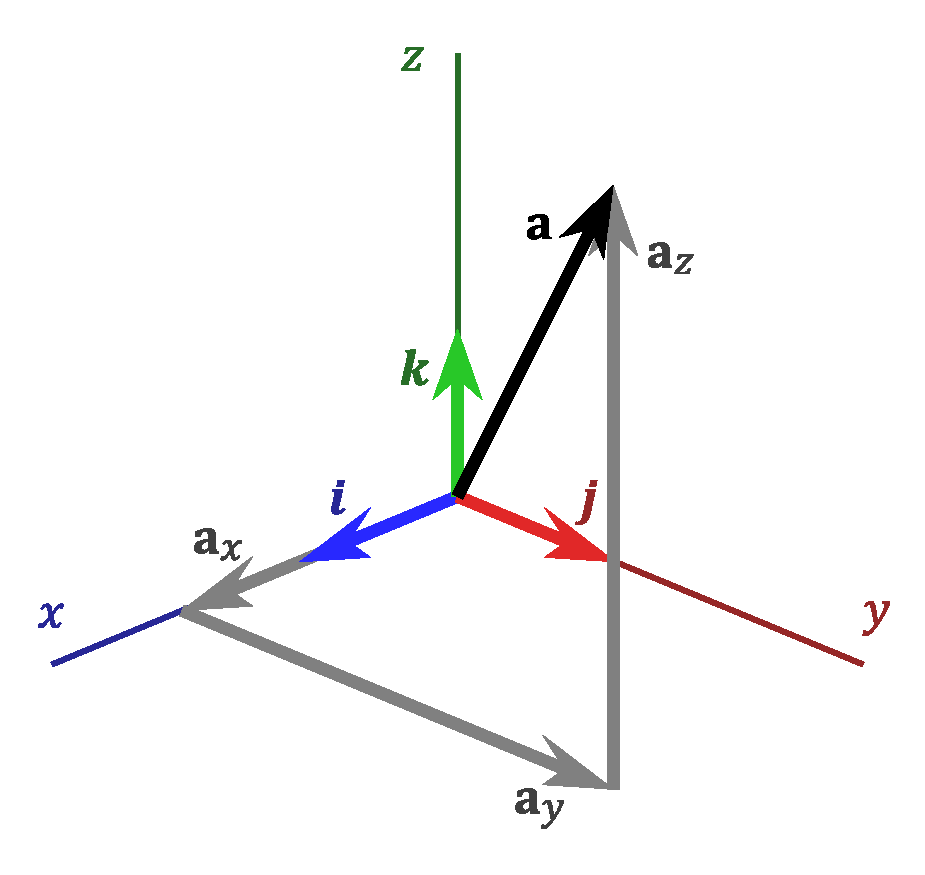
\includegraphics[width=0.8\onepicwidth]{figure/gbdt/3D_Vector}
        \caption{向量空间\footnote{
                 \href{https://en.wikipedia.org/wiki/Standard_basis}{Standard basis, Wikipedia}}}
    \end{figure}
\end{frame}

\begin{frame}
    \begin{figure}
        \centering
        \resizebox{1.1\onepicwidth}{!}{\begin{tikzpicture}
    [place/.style={circle,scale=0.3,draw=green!50,fill=green!20,thick},
    transition/.style={rectangle,draw=black!50,fill=black!20,thick}]

    \clip (-1,-6) rectangle (10,4);

    \draw[dotted] (0,0) circle [x radius=1.5, y radius=1];
    \draw[dotted] (0,0) circle [x radius=2.5, y radius=2];
    \draw[dotted] (0,0) circle [x radius=3.5, y radius=3];
    \draw[dotted] (0,0) circle [x radius=4.5, y radius=4];
    \draw (-3,0) node {$L(\cdot)$};

    \node[place,label=above:{$y_0=F_0(X)$}] (f0) at (1.8,3.24)  {};
    \node[place,label=north east:{$y_1$}] (f1) at (3.0,-0.3)  {};
    \node[place,label=below:{$y_2$}] (f2) at (1.0,-1.0)   {};
    \node[circle,draw=red,fill=red,scale=0.3] (f3) at (0.6,0.0)   {};
    \node[place,label=below:{$y$},label=north east:{$y_n$}] (fn) at (0,0)  {};

    \draw[->,>=stealth,dashed] (f0) -- (f1);
    \draw[->,>=stealth,dashed] (f1) -- (f2);
    \draw[->,>=stealth,dashed] (f2) -- (f3);
    \draw[->,>=stealth,dashed] (f3) -- (fn);

    \draw[help lines] (6.2,-3.8) grid (9.8, -0.8);
    \node[circle,scale=0.3,label=right:$X$,draw] (x) at (7.5,-2.5) {};
    \node[scale=0.3] (hx1) at (8.7,-6.04) {};
    \node[scale=0.3] (hx2) at (5.5,-3.2) {};

    \draw[arrow] (x) -- (f0)  node[midway,above] {$F_0$};
    \draw[arrow] (x) -- (hx1) node[below] {$h(x; \mathbf{a})$};
    \draw[arrow] (x) -- (hx2) node[left] {$h(x; \mathbf{a})$};

    \draw[arrow,red] (x) -- (f3) node[midway,above] {$F$};
    \draw[arrow,blue] (x) -- (fn) node[midway,below] {$F_n$};

    %\draw[arrow,dashed] (x) -- ($ (x) !.95! (f2)$) node[midway,below] {$F_2$};

    %\draw[arrow,blue] (x) -- (fn) node[near end,above] {$F_n$};

    %\draw (0,-6) node[scale=1.3] {$F_n(x) = F_{0}(x) + \sum_n \rho_m h(x; \mathbf{a}_m)$};
\end{tikzpicture}
}
    \end{figure}
\end{frame}

\begin{frame}
    泰勒展开:$\sum _{n=0}^{\infty }{\frac{f^{(n)}(a)}{n!}}\,\textcolor{blue}{(x-a)^{n}}$

    \begin{figure}[!tb]
        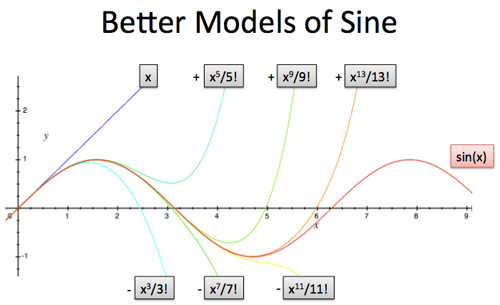
\includegraphics[width=\twopicwidth]{figure/gbdt/sine-better-models}
        \caption{sin函数泰勒展开示意\footnote{
                 \href{https://betterexplained.com/articles/intuitive-understanding-of-sine-waves/}{Intuitive Understanding of Sine Waves}}}
    \end{figure}

    GBDT: $F_n(x) = F_{0}(x) + \sum_n \rho_m \textcolor{blue}{h(x; \mathbf{a}_m)}$
\end{frame}


\subsection{从降维角度的理解}
% PCA
%% 数据特征的降维 -> 函数空间的降维
%% 矩阵分解
\begin{frame}
    \begin{figure}
        \centering
        \subfigure[][]{
            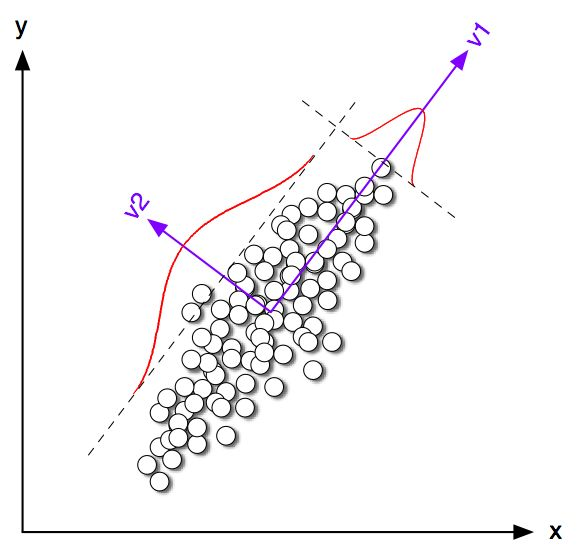
\includegraphics[width=0.40\linewidth]{figure/gbdt/PCA}
        }
        \hfil
        \subfigure[][]{
            \resizebox{0.50\linewidth}{!}{\begin{tikzpicture}
    [place/.style={circle,scale=0.3,draw=green!50,fill=green!20,thick},
    transition/.style={rectangle,draw=black!50,fill=black!20,thick}]

    \clip (-1,-6) rectangle (10,4);

    \draw[dotted] (0,0) circle [x radius=1.5, y radius=1];
    \draw[dotted] (0,0) circle [x radius=2.5, y radius=2];
    \draw[dotted] (0,0) circle [x radius=3.5, y radius=3];
    \draw[dotted] (0,0) circle [x radius=4.5, y radius=4];
    \draw (-3,0) node {$L(\cdot)$};

    \node[place,label=above:{$y_0=F_0(X)$}] (f0) at (1.8,3.24)  {};
    \node[place,label=north east:{$y_1$}] (f1) at (3.0,-0.3)  {};
    \node[place,label=below:{$y_2$}] (f2) at (1.0,-1.0)   {};
    \node[circle,draw=red,fill=red,scale=0.3] (f3) at (0.6,0.0)   {};
    \node[place,label=below:{$y$},label=north east:{$y_n$}] (fn) at (0,0)  {};

    \draw[->,>=stealth,dashed] (f0) -- (f1);
    \draw[->,>=stealth,dashed] (f1) -- (f2);
    \draw[->,>=stealth,dashed] (f2) -- (f3);
    \draw[->,>=stealth,dashed] (f3) -- (fn);

    \draw[help lines] (6.2,-3.8) grid (9.8, -0.8);
    \node[circle,scale=0.3,label=right:$X$,draw] (x) at (7.5,-2.5) {};
    \node[scale=0.3] (hx1) at (8.7,-6.04) {};
    \node[scale=0.3] (hx2) at (5.5,-3.2) {};

    \draw[arrow] (x) -- (f0)  node[midway,above] {$F_0$};
    \draw[arrow] (x) -- (hx1) node[below] {$h(x; \mathbf{a})$};
    \draw[arrow] (x) -- (hx2) node[left] {$h(x; \mathbf{a})$};

    \draw[arrow,red] (x) -- (f3) node[midway,above] {$F$};
    \draw[arrow,blue] (x) -- (fn) node[midway,below] {$F_n$};

    %\draw[arrow,dashed] (x) -- ($ (x) !.95! (f2)$) node[midway,below] {$F_2$};

    %\draw[arrow,blue] (x) -- (fn) node[near end,above] {$F_n$};

    %\draw (0,-6) node[scale=1.3] {$F_n(x) = F_{0}(x) + \sum_n \rho_m h(x; \mathbf{a}_m)$};
\end{tikzpicture}
}
        }
        \caption{PCA\footnotemark 比较示意}
    \end{figure}

    \footnotetext{\href{https://lazyprogrammer.me/tutorial-principal-components-analysis-pca/}{Tutorial: Principal Components Analysis (PCA)}}
\end{frame}

% 寻优耗时
% spark,实现,没有寻优 => tree boost
%% 用sklearn, spark代码引出Tree Boost
\begin{frame}[fragile]
    \begin{lstlisting}[language=Scala,style=myScalastyle]
def boost(
  // +-- 46 lines: input: RDD[LabeledPoint],------------------------------
  val firstTree = new DecisionTreeRegressor().setSeed(seed)
  val firstTreeModel = firstTree.train(input, treeStrategy)
  val firstTreeWeight = 1.0
  baseLearners(0) = firstTreeModel
  baseLearnerWeights(0) = firstTreeWeight
  // +-- 17 lines: var predError: RDD[(Double, Double)] =-----------------
  while (m < numIterations && !doneLearning) {
    // Update data with pseudo-residuals
    val data = predError.zip(input).map { case ((pred, _), point) =>
    LabeledPoint(-loss.gradient(pred, point.label), point.features)
    }
    // +--  5 lines: timer.start(s"building tree $m")----------------------
    val dt = new DecisionTreeRegressor().setSeed(seed + m)
    val model = dt.train(data, treeStrategy)
    baseLearners(m) = model
    baseLearnerWeights(m) = learningRate

    predError = updatePredictionError(
    input, predError, baseLearnerWeights(m), baseLearners(m), loss)
    // +-- 21 lines: predErrorCheckpointer.update(predError)---------------
    m += 1
  }
}
    \end{lstlisting}
    {\tiny \tt
    source: spark/ml/tree/impl/GradientBoostedTrees.scala \\[-2ex]
    commit: 2eedc00b04ef8ca771ff64c4f834c25f835f5f44}
\end{frame}
